\section{Implementing a prototypical micro-frontend architecture}\label{section:applied-methods:prototypical-implementation}

The first step was to implement a prototypical micro-frontend application to evaluate the hypothesis. The base architecture was developed to lay the groundwork for later use in a production environment. The micro-frontends are integrated using client-side integration, more precisely, run-time integration. The integration strategy was implemented with Webpack's Module Federation, which was described in more detail in Section \ref{subsection:background:micro-frontend:module-federation}. The majority of the implementation is written in Angular. One micro-frontend was implemented in React to showcase the technology agnosticism of the caching strategy. The prototype contains an application shell that consumes the other micro-frontends. The architecture is divided into nine widgets that display only simple data and four complex single-page applications. The four \acp{SPA} are Dashboard, Contact, Sales, and User.

\bigskip

\noindent The library Nx from the company Nwrl is used for managing the micro-frontends and libraries in a single monorepo. An essential feature of Nx is the support for monorepos, which is the perfect match for managing micro-frontend applications. It offers support and tooling for almost any \ac{JS} framework and can be customized with plugins. Multiple related projects can be managed in a single workspace. Additionally, it ensures that every project uses the same version of a dependency across the workspace. Besides, Nx offers helper functions for working with Module Federation in micro-frontends. \cite{misc:-:applied-methods:intro-to-nx}

\bigskip

\noindent A rough overview of the architecture is shown in Figure \ref{fig:applied-methods:prototype-micro-frontend-architecture}. It shows a wireframe of the structure of the application. The icons inside the squares represent the \ac{JS} framework used. Each widget is a separate micro-frontend that exposes a remote module through Module Federation, which is then consumed by the Dashboard micro-frontend.

\ifshowImages
\begin{figure}[H]
  \centering
  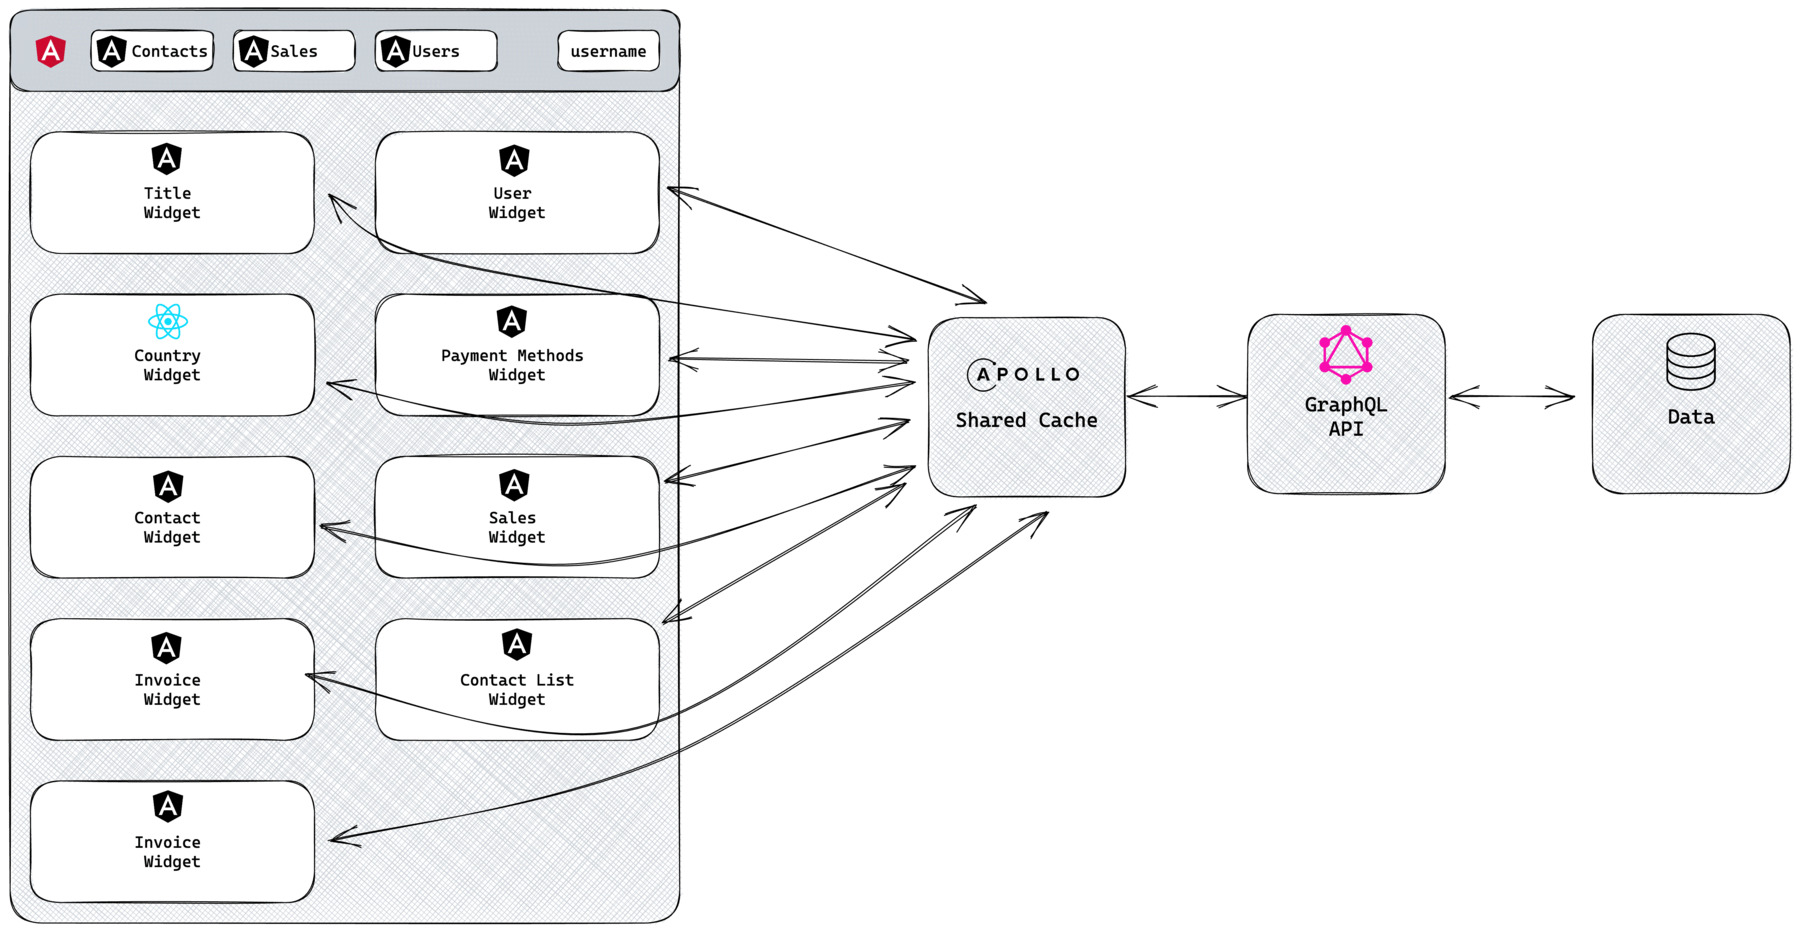
\includegraphics[width=1\linewidth]{images/applied-methods/prototypical-implementation/host-architecture.jpg}
  \caption{The architecture of the micro-frontend prototype.}\label{fig:applied-methods:prototype-micro-frontend-architecture}
\end{figure}
\fi

\noindent Each micro-frontend is deployed separately and is accessible by a separate \ac{URL}. The application shell is the entry point for the client, and it consumes the Dashboard, Contact, Sales, and User application. The main functionality of the micro-frontends is encapsulated in modules. These modules of the applications can be easily accessed through the Module Federation and used by the application shell. The modules are used in exactly the same way in the standalone application.

\bigskip

\noindent The Listing \ref{code:applied-methods:module-federation-config-expose} shows the configuration of the contact micro-frontend to expose its primary implementation through module federation in the form of the \texttt{entry.module}. The configuration of the other micro-frontends looks similar. The properties of the module-federation plugin were already discussed in Section \ref{subsection:background:micro-frontend:module-federation}. All Angular- and Apollo- dependencies are specified to be shared across all micro-frontends. Sharing the dependencies ensures that all micro-frontends use the same and only one version of the dependencies. Listing \ref{code:applied-methods:module-federation-config-expose}, the versions of the dependencies are explicitly specified. Inside the prototype, the versions are read from the root \texttt{package.json} to ensure consistency with the installed versions.

\ifshowListings
\begin{listing}[H]
  \begin{minted}{typescript}
module.exports = {
  name: 'contact',
  exposes: {
    './Module': 'apps/contact/src/app/remote-entry/entry.module.ts',
  },
  shared: [
    '@angular/core': {
      singleton: true, strictVersion: true, requiredVersion: '^15.1.1' 
    },
    ...
    'apollo-angular': { 
      singleton: true, strictVersion: true, requiredVersion: '^4.0.1' 
    },
    ...
  ]
};
  \end{minted}
  \caption{The Module Federation configuration to expose the contact's functionality.}\label{code:applied-methods:module-federation-config-expose}
\end{listing}
\fi

\noindent The application shell is configured to consume the remote modules listed inside the \texttt{remotes}-object. The configuration to consume the four micro-frontends of the architecture can be seen in the Listing \ref{code:applied-methods:module-federation-config-consume}. This configuration allows the application-shell to consume the \texttt{entry.module} of the remote applications, which were exposed before with the configuration from Listing \ref{code:applied-methods:module-federation-config-expose}. As with the remote module configuration, the application shell shares the same dependencies. Dependency sharing is required so that micro-frontends can load their runtime dependencies from the application shell and use the same dependency version.

\ifshowListings
\begin{listing}[H]
  \begin{minted}{typescript}
module.exports = {
  name: 'host',
  remotes: {
    contact: 'contact@http://localhost:4201/remoteEntry.js'
    sales: 'sales@http://localhost:4202/remoteEntry.js'
    dashboard: 'dashboard@http://localhost:4203/remoteEntry.js'
    user: 'user@http://localhost:4204/remoteEntry.js'
  },
  shared: {
    '@angular/core': {
      singleton: true, strictVersion: true, requiredVersion: '^15.1.1' 
    },
    ...
    'apollo-angular': { 
      singleton: true, strictVersion: true, requiredVersion: '^4.0.1' 
    },
    ...
  }
};
  \end{minted}
  \caption{The configuration of the application-shell to be able to consume micro-frontends.}\label{code:applied-methods:module-federation-config-consume}
\end{listing}
\fi

\noindent Using the Module Federation configuration from Listing \ref{code:applied-methods:module-federation-config-consume}, the application shell can load and display the remote modules. Listing \ref{code:applied-methods:angular-route-to-remote-module} shows the route configuration for displaying the contact micro-frontend using Angular's router. Nx offers helper methods like \texttt{loadRemoteModule} for Module Federation to load remote modules into a route of the application shell. The application shell follows the approach of showing one micro-frontend per route. The dashboard on the other hand displays multiple micro-frontend widgets on a page.

\ifshowListings
\begin{listing}[H]
  \begin{minted}{typescript}
const routes: Routes = [
  {
    path: 'contact',
    loadChildren: () => loadRemoteModule('contact', './Module')
      .then((m) => m.ContactRemoteEntryModule),
  },
  ...
]
  \end{minted}
  \caption{An Angular route to the contact application.}\label{code:applied-methods:angular-route-to-remote-module}
\end{listing}
\fi

\ifshowAppliedMethodsCustomNginxConfSection
  \subsection{Deployment problems}\label{subsection:applied-methods:prototypical-implementation:nginx-problems}

Docker is used to run the micro-frontends in production. The Nginx web server in a Docker container is used to deliver the application files to the client. The dockerfile for the micro-frontends is shown in Listing \ref{code:applied-methods:prototype-implementation-dockerfile}. The application to deploy needs to be built before creating the docker image. Afterwards the necessary files are copied into the docker image.

\ifshowListings
  \begin{listing}[H]
  \begin{minted}{dockerfile}
FROM nginx:alpine
COPY nginx/nginx.conf /etc/nginx/nginx.conf
COPY dist/apps/contact/ /usr/share/nginx/html/
    
CMD [
  "/bin/sh", 
  "-c", 
  "envsubst < /usr/share/nginx/html/assets/settings.template.json >" 
  "/usr/share/nginx/html/assets/settings.json && exec nginx -g daemon off;"
]
  \end{minted}
  \caption{The dockerfile for containerizing a micro-frontend.}\label{code:applied-methods:prototype-implementation-dockerfile}
  \end{listing}
\fi

\noindent Module Federation applications expose a file called \texttt{remoteEntry.mjs}, which is consumed by an application shell. However, Nginx currently cannot interpret the mime-type of \texttt{\*.mjs} files which would be \ac{JS}. Therefore, it falls back to the default mime-type \texttt{text/plain}, where \ac{JS} is not executed in the browser. As a workaround for this problem, a custom \texttt{nginx.conf} has been created that sets the default mime-type to \texttt{text/javascript}, which allows the execution of the script in the browser. A part of the configuration is shown in Listing \ref{code:applied-methods:prototype-implementation-custom-nginx-conf}.

\ifshowListings
  \begin{listing}[H]
  \begin{minted}{bash}
default_type text/javascript;
  \end{minted}
  \caption{The custom configuration for Nginx to set the default mime type.}\label{code:applied-methods:prototype-implementation-custom-nginx-conf}
  \end{listing}
\fi

\noindent The custom configuration allows Nginx to correctly load and interpret the remote module files. Setting another default mime type will not break the web server because modern frameworks like Angular just work with \ac{JS} files.

\fi

\subsection{Integrating the React micro-frontend}\label{subsection:applied-methods:prototypical-implementation:react-micro-frontend}

One widget for the dashboard micro-frontend was implemented using the popular frontend framework React. Implementing one micro-frontend in another technology was done to show that the concept of sharing a single cache instance between multiple micro-frontends is technology agnostic. The React widget exposes its functionality like the Angular counterparts through Module Federation. In comparison to Angular, React does not have the concept of modules. Therefore, the functionality of the widget is exported as a simple, functional React component, as shown in listing  \ref{code:applied-methods:module-federation-react-config-expose}.

\ifshowListings
\begin{listing}[H]
    \begin{minted}{typescript}
module.exports = {
  name: 'react-dashboard',
  exposes: { './Module': './src/remote-entry.ts' },
  shared: [
    react: {
      singleton: true, strictVersion: true, requiredVersion: '^18.2.0' 
    },
    ...
  ]
};
    \end{minted}
    \caption{Module Federation config for exposing the \texttt{remote.entry} of the React micro-frontend.}\label{code:applied-methods:module-federation-react-config-expose}
\end{listing}
\fi

\noindent The host application can consume the React application in the same way as the Angular remote modules. However, rendering a React component in an Angular application is natively impossible. Therefore, an Angular wrapper component loads the React remote bundle and renders it inside an HTMLElement. The Angular adapter makes it possible for the Angular router to point to the component, which is impossible with the React component directly.

\bigskip

\noindent Angular modules consumed through Module Federation can access the \ac{DI} tree from the application shell. However, React does not offer a \ac{DI} system like Angular and cannot access the necessary dependencies. React uses contexts to pass down data through the component tree without manually passing properties down level by level. It enables data sharing between components not directly connected in the component tree. The make the shared caching layer inside the React application work, the React widget needs the \texttt{InMemoryCache} instance from the application shell. The shared caching layer is explained in Section \ref{section:applied-methods:shared-caching-layer} in more detail, but the general concept is needed to understand the need to incorporate the instance into the React context. Therefore, the Angular wrapper creates the exposed widget inside a React context provider with the necessary dependencies. The function in listing \ref{code:applied-methods:prototypical-implementation:render-react-component-with-context} shows the React context provider's creation and the React component's rendering. 

\ifshowListings
\begin{listing}[H]
    \begin{minted}{typescript}
render<Comp extends ElementType>(rootEl: Root, Comp: Comp) {
  rootEl.render(
    createElement(
      NgReactContext, {
        ctx: {
          graphQLClientCache: this.injector.get(GRAPHQL_CLIENT_CACHE),
          ...
        },
      },
      createElement(Comp, compProps)
    )
  );
}
    \end{minted}
    \caption{The function to render the React widget into an Angular component.}\label{code:applied-methods:prototypical-implementation:render-react-component-with-context}
\end{listing}
\fi

\noindent With the help of the function, the widget can access the instance of the \texttt{InMemoryCache} from the application shell and use it to share the cache between the Angular and the React micro-frontend. How the \texttt{InMemoryCache} from the application shell is injected and consumed is shown in listing \ref{code:applied-methods:prototypical-implementation:consume-react-context}. The cache is used to create a new instance of the ApolloClient, and afterwards the client is provided to the application using another context.

\ifshowListings
\begin{listing}[H]
    \begin{minted}{typescript}
const injector = useContext(InjectorCtx);

const client = new ApolloClient({
  uri: injector.graphQLEndpoint,
  cache: injector.graphQLClientCache,
  ...
});

return (
  <ApolloProvider client={client}>
    <PaymentMethodList />
  </ApolloProvider>
);

    \end{minted}
    \caption{Use the \texttt{InMemoryCache} instance from the React context.}\label{code:applied-methods:prototypical-implementation:consume-react-context}
\end{listing}
\fi


\subsection{Backend for frontend}\label{subsection:background:prototypical-implemenation:bff}

The \ac{BFF} pattern was implemented using GraphQL. A single \ac{BFF} service is used for all micro-frontends of the architecture. Apollo Server is used as the GraphQL server and was chosen to implement the \ac{API}. Every micro-frontend uses the same \ac{BFF} service, however, multiple GraphQL \acp{API} could be used. Each micro-frontend is a standalone application, therefore it could communicate with multiple GraphQL \acp{API}.
The GraphQL \ac{API} fetches the data from a cluster of microservices and brings the results into the correct shape for the micro-frontends. The GraphQL \ac{API} was developed, while the microservices were still under development. However, the data model was already finalized. Therefore, the GraphQL \ac{API} was implemented using mock data. The mock data was generated using the database schemas of the microservices. The queries and mutations were implemented by directly reading and writing the mock data. Once the microservices are implemented, the GraphQL \ac{API} will be modified to communicate directly with the microservices within the company.


\ifshowAppliedMethodsLoadRemoteSettingsSection
  \subsection{Remote application configuration}\label{subsection:applied-methods:prototypical-implementation
:load-remote-settings}

The application shell is set up to use dynamic Module Federation. The location of the remote applications is determined at runtime. The problem with the so-called static Module Federation is that the \ac{URL} of the remote application must be known at build time. However, this is troublesome if the application should be built once and deployed to multiple stages. It is very cumbersome to build an artifact for every environment.

\bigskip

\noindent One possibility to fetch the remote definitions at runtime is to store them in a simple \ac{JSON} file, which can easily be configured for every environment. The host makes a simple GET request to get the definitions inside the \ac{JSON} file. The content of the file has to be a simple mapping between the name of the remote and their location, as shown in Listing \ref{code:applied-methods:define-module-federation-manifest}.

\ifshowListings
\begin{listing}[H]
\begin{minted}{json}
{
  "sales": "http://localhost:4201",
  "contact": "http://localhost:4202",
  "dashboard": "http://localhost:4203",
  "user": "http://localhost:4204"
}
\end{minted}
\caption{The structure of the micro-frontend definition file with the name and \ac{URL}.}\label{code:applied-methods:define-module-federation-manifest}
\end{listing}
\fi

\noindent The host has to fetch the definitions when starting up the application. The definitions are stored and stored for the Webpack configuration, as shown in Listing \ref{code:applied-methods:load-module-federation-settings}. If the file can be fetched successfully, the bootstrap process of the application gets imported dynamically.

\ifshowListings
\begin{listing}[H]
\begin{minted}{typescript}
fetch('/assets/module-federation.manifest.json')
  .then((res) => res.json())
  .then((definitions) => setRemoteDefinitions(definitions))
  .then(() => import('./bootstrap').catch((err) => console.error(err)));
\end{minted}
\caption{Loading the micro-frontend definition file during initialization.}\label{code:applied-methods:load-module-federation-settings}
\end{listing}
\fi

\noindent Another use case for dynamic content is the configuration of an application. This configuration includes the endpoint of the GraphQL \ac{API}, which can be different in staging and production. Therefore, the configuration should also be fetched dynamically. The settings are fetched during the first load of the application and stored for later use. The configuration is stored inside a file called \texttt{settings.json}, served alongside the application. Angular provides a handy mechanism to run code when the application is loaded.

\bigskip

\noindent With the help of the \texttt{APP\_INITIALIZER} injection token, asynchronous code can be executed when the application starts up. Such tasks include fetching data from a remote \ac{API} and setting up configuration or initializing third-party libraries. When an Angular app starts, it will execute all the functions registered with \texttt{APP\_INITIALIZER} in the order they were defined. If one of the initialization tasks fails, the application will not load. \cite{misc:-:applied-methods:prototype-implementation:angular-app-initializer}

\bigskip

\noindent The Listing \ref{code:applied-methods:fetch-and-store-settings} shows a simplified version to fetch and store the settings in the local storage. The settings are fetched from the \texttt{settings.json} file, which content is used to configure the application. The settings of the application shell are stored with the key \texttt{host}. Each application of the micro-frontend architecture stores its settings with its application name as the key.

\ifshowListings
\begin{listing}[H]
\begin{minted}{typescript}
@NgModule({
  providers: [{
    provide: APP_INITIALIZER,
    async useFactory(http: HttpClient, storage: StorageClient) {
      const environmentConfig = await lastValueFrom(
        http.get('assets/settings.json')
      );
      storage.store('host', environmentConfig);
    },
    multi: true,
    deps: [HttpClient, StorageClient],
  }]
})
class CoreModule {}
\end{minted}
\caption{Fetch \& store the settings of the application shell.}\label{code:applied-methods:fetch-and-store-settings}
\end{listing}
\fi

\subsubsection{Loading the configuration of the remote applications}\label{subsubsection:applied-methods:prototypical-implementation
:load-the-configuration}

Each application of the prototypical micro-frontend architecture follows this approach. When the application is initialized, the application configuration is fetched with a GET request from the \texttt{settings.json}. As mentioned in the previous section, each micro-frontend stores its settings with the application's name as the key. However, the configuration does not get fetched when the application shell consumes the functionality of a micro-frontend. Therefore, the application throws errors because they cannot access their settings from the storage. To solve the problem of missing settings for the application, the configuration of a remote application is fetched and stored inside a store when the user navigates to it. This procedure is explained visually in Figure \ref{fig:applied-methods:load-remote-settings}.

\ifshowImages
  \begin{figure}[H]
  \centering
  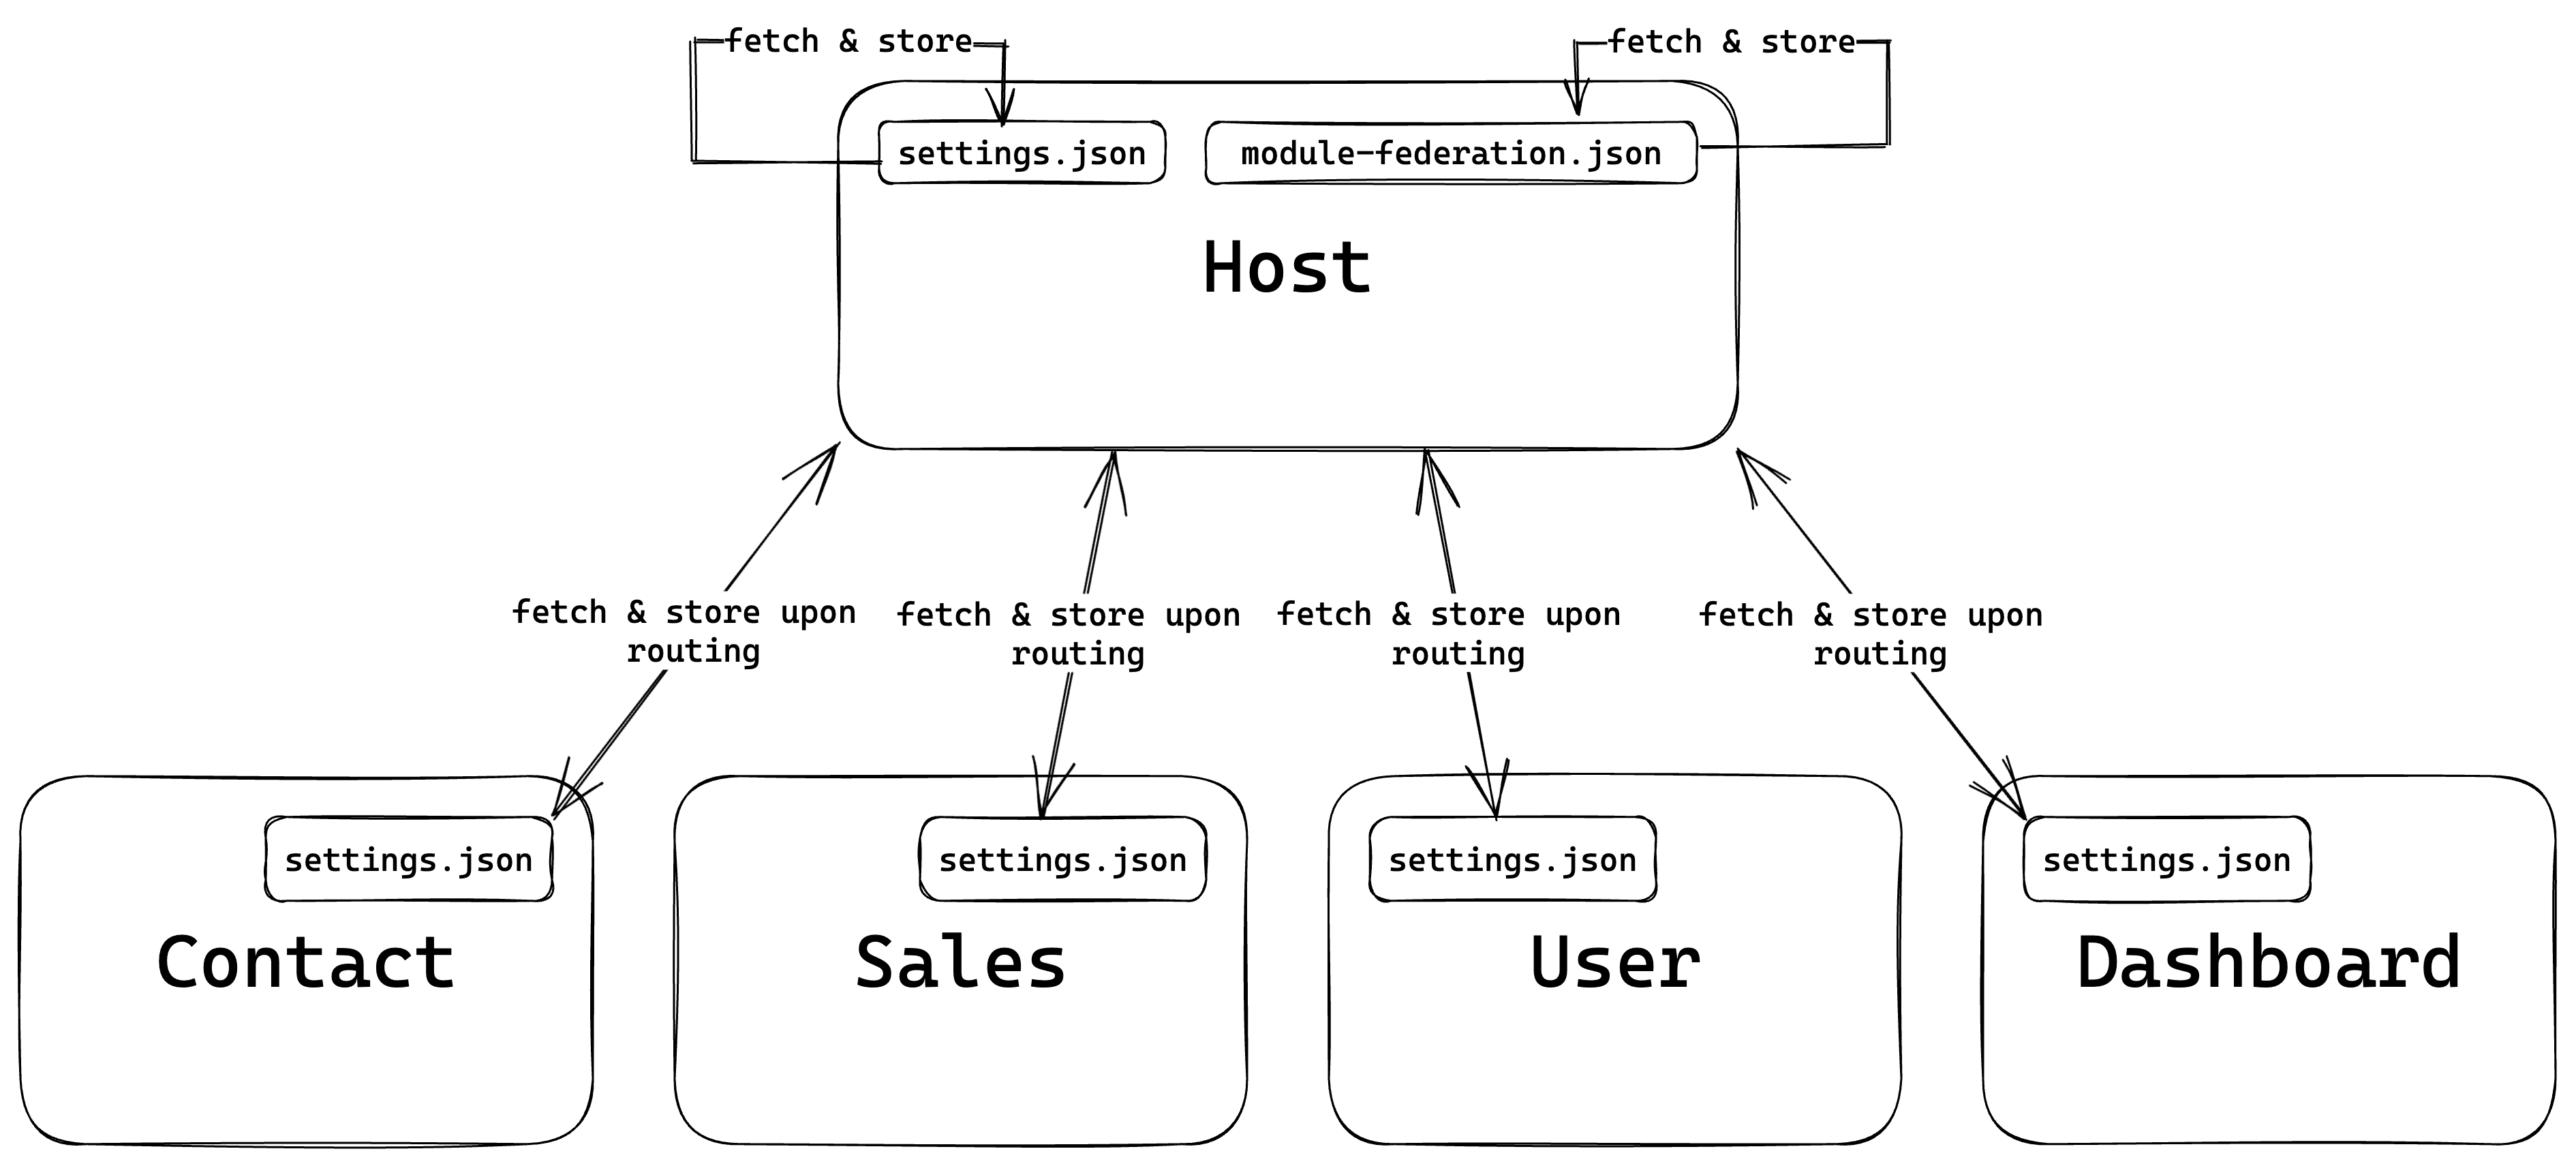
\includegraphics[width=0.9\linewidth]{images/applied-methods/prototypical-implementation/load-remote-settings.png}
  \caption{Loading a storing the configuration of the remote applications.}\label{fig:applied-methods:load-remote-settings}
  \end{figure}
\fi

\noindent With the help of Angular resolvers, the resolvers executed before the components of the target are rendered. Due to the dynamic Module Federation, the location of the remote module is known. Therefore, the \texttt{settings.json} is loaded and stored in addition to loading the remote module. A simplified version of the code is shown in Listing \ref{code:applied-methods:fetch-and-store-remote-application-settings}. The same principle applies to every remote module, which is consumed.

\ifshowListings
\begin{listing}[H]
\begin{minted}{typescript}
const routes: Routes = [{
    path: 'contact',
    loadChildren: () => loadRemoteModule('contact', './Module')
      .then((m) => m.ContactRemoteEntryModule),
    resolve: {
      settings: () => {
        const contact = inject(StorageClient).get('manifest')['contact'];
        return inject(HttpClient).get(`\${contact}/assets/settings.json`);
      }
    },
  },
  ...
]
\end{minted}
\caption{Fetch the settings of the contact application.}\label{code:applied-methods:fetch-and-store-remote-application-settings}
\end{listing}
\fi

\noindent With this approach, each application can access its settings like running in standalone mode. Moreover, it has another benefit because each application can only access its settings and not the settings of the other applications. 

\fi

\ifshowAppliedMethodsSecondaryEntrypoints
  \subsection{Sharing secondary entry points}\label{subsection:applied-methods:prototypical-implementation:sharing
-secondary-entrypoints}

By default, all dependencies of the micro-frontends are shared through Module Federation. The configuration options for every dependency are \texttt{singleton}-, \texttt{strictVersion}-, and \texttt{requiredVersion}-property. These properties are explained in more detail in Section \ref{subsection:background:micro-frontend:module-federation}. The versions of these dependencies are determined automatically from the \texttt{package.json}. However, not all packages support being shared with these default settings. The npm package \texttt{@apollo/client} has a problem because it has secondary entry points. When trying to share \texttt{@apollo/client/core}, \texttt{@apollo/client/link/batch} and \texttt{@apollo/client/link/error} the error message in Figure \ref{fig:applied-methods:sharing-secondary-entrypoints-error} is shown.

\ifshowImages
  \begin{figure}[H]
  \centering
  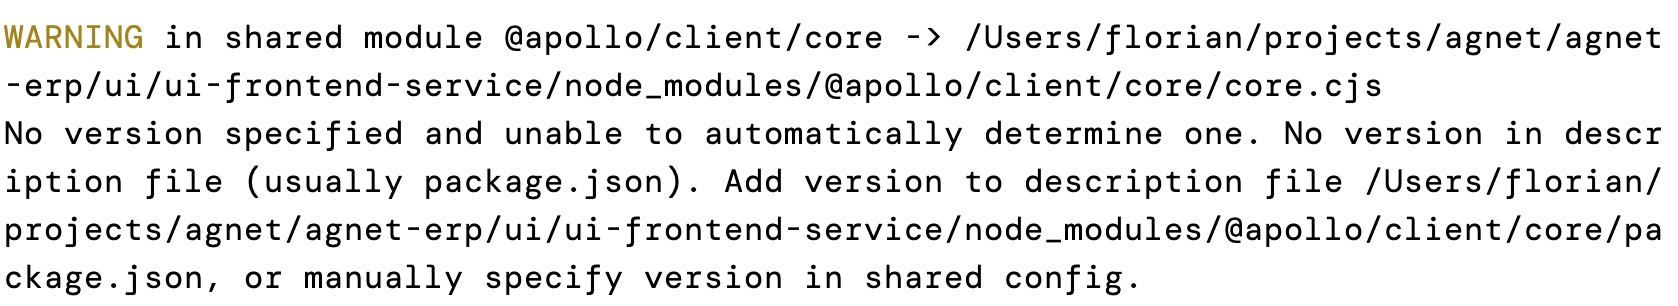
\includegraphics[width=1\linewidth]{images/applied-methods/prototypical-implementation/module-federation-apollo-warning.jpg}
  \caption{A Module Federation warning, when the dependency \texttt{@apollo/client} should be shared.}\label{fig:applied-methods:sharing-secondary-entrypoints-error}
  \end{figure}
\fi

\noindent The problems are secondary entry points like \texttt{@apollo/client/core}, which are a bit like an npm package in another npm package. The \texttt{package.json} of \texttt{@apollo/client/core} is shown in Listing \ref{code:applied-methods:package-json-apollo-client-core}. Webpack tries to resolve the version of the secondary entry point from the \texttt{package.json} and not from \texttt{@apollo/client}. Therefore, it cannot determine the version and prints the warning shown in Figure \ref{fig:applied-methods:sharing-secondary-entrypoints-error}. The warning does not lead to an error, but these dependencies cannot be shared and must be included in every micro-frontend bundle.

\ifshowListings
\begin{listing}[H]
  \begin{minted}{json}
{
  "name": "@apollo/client/core",
  "type": "module",
  "main": "error.cjs",
  "module": "index.js",
  "types": "index.d.ts",
  "sideEffects": false
}
  \end{minted}
  \caption{The \texttt{package.json} of \texttt{@apollo/client/core}.}\label{code:applied-methods:package-json-apollo-client-core}
\end{listing}
\fi

\noindent The Module Federation was fixed by specifying the version for these packages manually. The version is the same as that of \texttt{@apollo/client}. The configuration for the sharing of these packages is shown in the Listing \ref{code:applied-methods:sharing-secondary-entrypoints-config}. 

\ifshowListings
\begin{listing}[H]
  \begin{minted}{typescript}
shared: (libraryName, defaultConfig) => {
  if (libraryName.includes(`@apollo/client/`))
    return { ...defaultConfig, version: '^3.6.9' };

  return defaultConfig;
}
  \end{minted}
  \caption{Specify the version for the secondary entry points for the \texttt{@apollo/client} package.}\label{code:applied-methods:sharing-secondary-entrypoints-config}
\end{listing}
\fi

\fi